\section{Landau--Zener Surface Hopping}\label{sec:landau_zener}
We now move to a slightly different approach to nonadiabatic dynamics. Instead of propagating the electronic wavefunction along with the nuclear trajectories, we will use a solution of a simplified two-state problem to determine the population transfer. The \gls{lz} model is a simple model for nonadiabatic transitions between two electronic states during a nuclear passage through an avoided crossing. The total population transfer between the two states is then used to determine the probability of a surface hop. This approach is known as \gls{lzsh}. This idea seems very approximative, since we do not need the \gls{tdc} or the electronic wavefunction at all. However, it has been shown that \gls{lzsh} can yield results comparable to \gls{fssh} in variety of cases, while being computationally much cheaper. \supercite{10.1021/acs.jctc.0c00512}

The \gls{lz} model, first proposed by Landau, Zener, Stueckelberg, and Majorana in 1932,\supercite{10.1016/B978-0-08-010586-4.50014-6,10.1098/rspa.1932.0165,10.5169/seals-110177,10.1007/BF02960953} is an exact solution to \gls{tdse} with the time-dependent Hamiltonian in the diabatic representation given by
\begin{equation}\label{eq:landau_zener_hamiltonian}
H^{\symrm{dia}}=\frac{1}{2}\begin{pmatrix}
\alpha t&g\\
g&-\alpha t
\end{pmatrix},
\end{equation}
where $\alpha$ is the rate of change of the energy difference between the two diabatic states, and $g$ is the time-independent coupling between them. For simplicity, we will also define $E_1=\frac{1}{2}\alpha t$ and $E_2=-\frac{1}{2}\alpha t$. The wavefunction is expressed as a linear combination of the two diabatic states $\ket{\tilde{\phi}_1}$ and $\ket{\tilde{\phi}_2}$ in the interaction picture as
\begin{equation}
\ket{\Psi(t)}=Ae^{-\i\int^tE_1\dt}\ket{\tilde{\phi}_1}+Be^{-\i\int^tE_2\dt}\ket{\tilde{\phi}_2},
\end{equation}
where $A$ and $B$ are time-dependent coefficients. The integrals in the exponents are simply phase factors that will simplify some of the following equations. The lower boundary for the integrals is not important, since we just want it to be some arbitrary primitive function of $E_1$ and $E_2$ respectively. Inserting this wavefunction into the \gls{tdse} leads to the coupled differential equations for $A$ and $B$
\begin{align}
\dot A&=-\i\frac{g}{2}Be^{\i\int^tE_{12}\dt}\\
\dot B&=-\i\frac{g}{2}Ae^{-\i\int^tE_{12}\dt},
\end{align}
where $E_{12}=E_1-E_2=\alpha t$. After differentiating both equations once more and some algebraic manipulations, we arrive at the decoupled second-order differential equations
\begin{align}
\ddot A-\i\alpha t\dot A+\frac{g^2}{4}A&=0\\
\ddot B+\i\alpha t\dot B+\frac{g^2}{4}B&=0.\label{eq:landau_zener_uncoupled_b}
\end{align}
Zener solved these equations by transforming them into the Weber equations, whose solutions are known as parabolic cylinder functions.\supercite{10.1017/9781009004091} We will use a more modern approach described by Wittig.\supercite{10.1021/jp040627u} We will assume our system is initially in state $\ket{\tilde{\phi}_2}$, which means that $A(t\to-\infty)=0$ and $B(t\to-\infty)=1$. The goal is to obtain final populations at $t\to\infty$.

Let's start by rewriting Eq.~\eqref{eq:landau_zener_uncoupled_b} in an integral form
\begin{equation}
\i\alpha\int_1^{B_f}\frac{\symrm{d}B}{B}=-\frac{g^2}{4}\int_{-\infty}^\infty\frac{\dt}{t}-\int_{-\infty}^\infty\frac{1}{t}\frac{\ddot B}{B}\dt,
\end{equation}
where $B_f=B(t\to\infty)$. Obviously, if we considered real time $t$, the integral $\int_{-\infty}^\infty\frac{\dt}{t}$ would not be defined. However, we can avoid this problem by considering complex time and integrating along a contour that avoids the singularity at $t=0$. The integral on the left-hand side can be evaluated as $\ln(B_f)$. The first integral on the right-hand side can be evaluated using a semicircular contour, yielding $\pm \i\pi$, where the sign depends on how we choose to avoid the singularity. With these results, we have
\begin{equation}
\i\alpha\ln(B_f)=\mp\i\pi\frac{g^2}{4}-\int_{-\infty}^\infty\frac{1}{t}\frac{\ddot B}{B}\dt.
\end{equation}
Now we have one integral left to evaluate. To evaluate it, we will need to inspect the asymptotic behavior of $\frac{\ddot B}{B}$ in the complex plane. Should we assume that $\ddot B$ is negligible to the other terms in Eq.~\eqref{eq:landau_zener_uncoupled_b} when $\lvert t\rvert\to\infty$, we can find asymptotic solution $B(t)\sim t^{i\gamma}$ where $\gamma=\frac{g^2}{4\alpha}$. But is this assumption valid? If we insert this asymptotic solution back into Eq.~\eqref{eq:landau_zener_uncoupled_b}, we find that $\dot B(t)\sim t^{-1}t^{i\gamma}$ and $\ddot B(t)\sim t^{-2}t^{i\gamma}$ which makes the first term in Eq.~\eqref{eq:landau_zener_uncoupled_b} negligible compared to the other two terms. So our assumption is valid, and we can use this asymptotic solution to evaluate the remaining integral.

Since we now know that the integrand of the remaining integral behaves as $\frac{1}{t}\frac{\ddot B}{B}\sim t^{-3}$ when $\lvert t\rvert\to\infty$, we can evaluate the integral using same semicircular contour as before. The contribution from the semicircle vanishes, and we are left with the integral along the real axis. The integral is now equivalent to the residue of the integrand at $t=0$ times $2\pi\i$
\begin{equation}
\int_{-\infty}^\infty\frac{1}{t}\frac{\ddot B}{B}\dt=\pm2\pi\i\,\symrm{Res}\left(\frac{1}{t}\frac{\ddot B}{B},0\right)\delta=\pm2\pi\i\frac{\ddot B(0)}{B(0)}\delta=\mp2\pi\i\frac{g^2}{4}\delta,
\end{equation}
where $\delta=1$ when the contour contains the singularity and $\delta=0$ otherwise. Inserting this result back into the previous equation, we have
\begin{equation}
\i\alpha\ln(B_f)=\mp\i\pi\frac{g^2}{4}\pm2\pi\i\frac{g^2}{4}\delta\implies B_f=\exp\left(\mp\frac{\pi g^2}{4\alpha}(1-2\delta)\right).
\end{equation}
Now, we want our final probability to be between 0 and 1, which means that we have to choose the contour such that $\delta=1$ and the sign in the exponent is positive or $\delta=0$ and the sign in the exponent is negative. This leaves us with the integration contours shown in Fig.~\ref{fig:landau_zener_contours}.
\begin{figure}[!ht]
\centering
\begin{subfigure}{.5\textwidth}
\centering
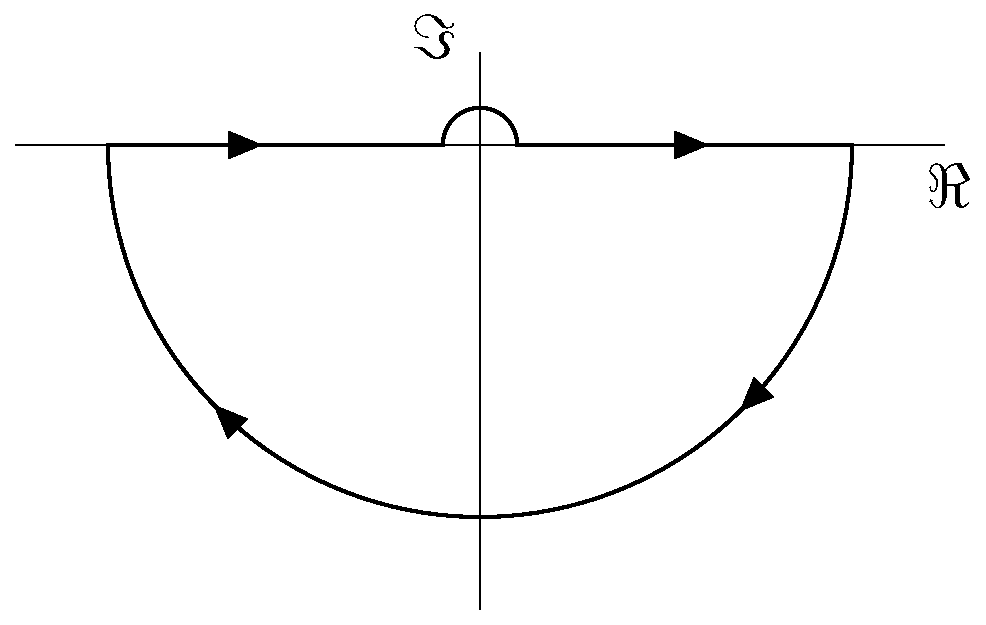
\includegraphics[width=.9\linewidth]{parts/01-Theoretical_Foundations/chapters/03-Mixed_Quantum-Classical_Dynamics/sections/images/lz_contour_counterclockwise}
\end{subfigure}\begin{subfigure}{.5\textwidth}
\centering
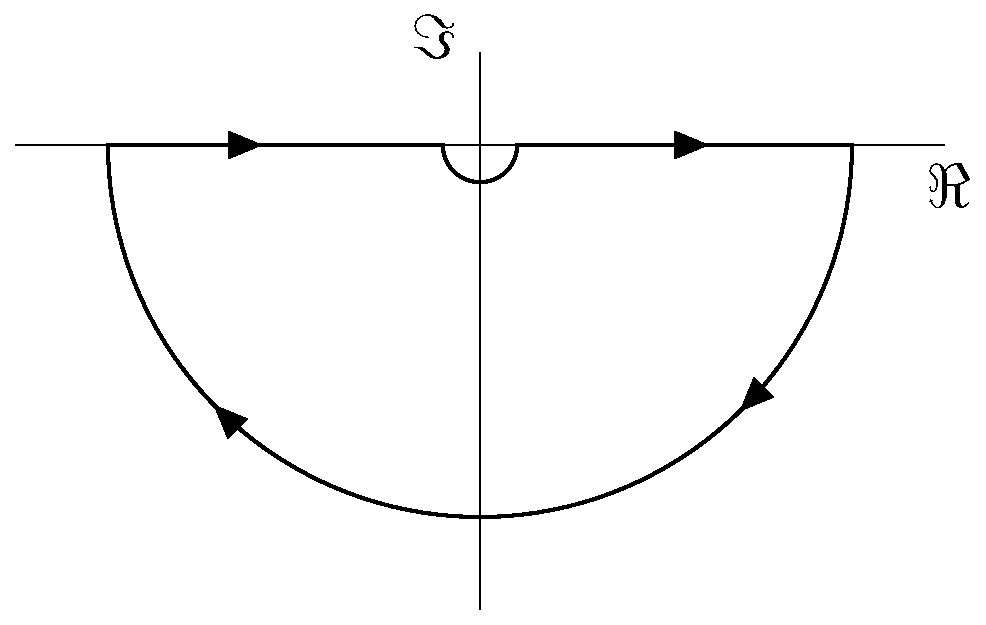
\includegraphics[width=.9\linewidth]{parts/01-Theoretical_Foundations/chapters/03-Mixed_Quantum-Classical_Dynamics/sections/images/lz_contour_clockwise}
\end{subfigure}
\caption{Possible integration contours in the complex time plane for evaluating the \gls{lz} transition probability. Both contours yield the same result for the final population transfer.}
\label{fig:landau_zener_contours}
\end{figure}
Both of these contours yield the same result for the final population transfer. Thus, we obtained the final probability of nonadiabatic transition as
\begin{equation}
P=\lvert B_f\rvert^2=e^{-2\pi\delta},
\end{equation}
where $\delta=\frac{g^2}{4\alpha}$. Since we have defined the population transfer probability as the final population of state $\ket{\tilde{\phi}_1}$ given that the system started in state $\ket{\tilde{\phi}_2}$, in surface hopping simulations, we can use this probability to determine whether a surface hop occurs when the nuclear trajectory passes through the crossing region.
\subsection{The Adiabatic Landau--Zener Formula}
In practical applications, we usually do not have access to the diabatic representation of the electronic states. Therefore, it is useful to express the \gls{lz} formula in the adiabatic representation. To do this, we need to first express the Hamiltonian in Eq.~\eqref{eq:landau_zener_hamiltonian} in the adiabatic representation as
\begin{equation}
H=\begin{pmatrix}
-\frac{1}{2}\sqrt{(\alpha t)^2+g^2}&0\\
0&\frac{1}{2}\sqrt{(\alpha t)^2+g^2}
\end{pmatrix}.
\end{equation}
We also define the adiabatic energy gap $Z_{21}=\sqrt{(\alpha t)^2+g^2}$, which is the same quantity as defined in Sec.~\ref{sec:baeck_an}. As mentioned in the diabatic case, in surface hopping simulations, we need to evaluate the \gls{lz} transition probability when the nuclear trajectory passes through the crossing region. This crossing region corresponds to the minimum energy gap, which occurs at $t=0$. To express all the diabatic parameters with the adiabatic energy difference $Z_{21}$ we differentiate $Z_{21}$ twice with respect to time to obtain
\begin{equation}
\ddot Z_{21}=\frac{\alpha^2Z_{21}-\alpha^2t\dot Z_{21}}{Z_{21}^2}.
\end{equation}
Using this expression and the definition of $Z_{21}$, we can express the probability of nonadiabatic transition in the adiabatic representation as
\begin{equation}\label{eq:landau_zener_adiabatic_2to1}
P_{2\to1}=\left.\exp\left(-\frac{\pi}{2}\sqrt{\frac{Z_{21}^3}{\ddot Z_{21}}}\right)\right\rvert_{t=0}
\end{equation}
Now, this is still the probability of transition between two states with a very specific Hamiltonian. However, in practical applications, we can approximate the energy gap $Z_{21}$ near the crossing region as a linear function of time and use the above formula to evaluate the transition probability. So instead of evaluating the probability $t=0$, we can evaluate it at the time $t_c$ when the energy gap is minimum along the nuclear trajectory. Thus, we arrive at the final form of the adiabatic \gls{lz} formula used in surface hopping simulations\supercite{10.1103/PhysRevA.84.014701}
\begin{equation}\label{eq:landau_zener_adiabatic}
P_{J\to I}=\left.\exp\left(-\frac{\pi}{2}\sqrt{\frac{Z_{JI}^3}{\ddot Z_{JI}}}\right)\right\rvert_{t=t_c}
\end{equation}
where $I$ and $J$ are the indices of the two states involved in the nonadiabatic transition and $t_c$ is the time when the energy gap between these two states is minimum along the nuclear trajectory. The extension to multiple states was purely heuristic, as the original \gls{lz} model only describes a two-state system. However, it has been shown that this extension works well in practice.\supercite{10.1021/acs.jctc.0c00512}

As one can see, the \gls{lz} formula does not introduce the need for electronic wavefunction coefficients. This, however, means that using this theory, we cannot capture the coherence between the electronic states, which can be limiting in some cases. This issue is investigated in more detail in one of my works in Sec.~\ref{sec:coherence_in_sh}.
\subsection{Practical Considerations and Multistate Extension}\label{sec:landau_zener_practical_considerations}
As mentioned before, the \gls{lz} formula was derived for a very specific two-state model. In practical applications, we need to make some approximations to apply it to more general systems. What, for example, should we do if we encounter a crossing region involving more than two states? In this case, the sum of the transition probabilities from one state to all the other states can exceed 1, which is unphysical. To avoid this problem, I have suggested and analyzed multiple ways to extend the \gls{lz} formula to multiple states in Ref.~\cite{10.1021/acs.jctc.5c01176}. The study converges on the following extension of the \gls{lz} formula to multiple states.

When the particle on state $I$ encounters a crossing region with multiple states, meaning the function $Z_{IJ}$ and $Z_{IK}$ have a minimum at the same time $t$, we evaluate the transition probability to a state with maximum second derivative of the energy gap. Meaning if $\ddot Z_{IJ}>\ddot Z_{IK}$, we evaluate the transition probability to state $J$ and proceed as if it was a two-state crossing. This approach is, of course, fully empirical, but it has been shown to work well in our study.

Another practical problems with the \gls{lz} formula is the need for numerical derivatives of the energy gap. If the \glspl{pes} are discontinuous, which is often the case in real systems, the numerical derivatives are ill-defined, which can lead to spurious hops and inaccurate results. To avoid this problem, we have suggested an algorithm that can recognise false minima in the energy gap and avoid evaluating the \gls{lz} formula at these points. This algorithm is described in detail also in Ref.~\cite{10.1021/acs.jctc.5c01176} and has been shown to work well in practice. The algorithm works as follows.

If \gls{lzsh} finds a minimum in $Z_{IJ}$, it compares numerical second derivatives of $Z_{IJ}$ at the minimum ($\ddot Z_{IJ,\symrm{min}}$) and at the previous step ($\ddot Z_{IJ,\mathrm{prev}}$). In the case of an avoided crossing, these second derivatives should vary smoothly. However, if a discontinuity is encountered, an abrupt change in the second derivative is expected. Therefore, we define a ratio $\alpha=\left\lvert\frac{\ddot Z_{IJ,\symrm{min}}-\ddot Z_{IJ,\mathrm{prev}}}{\ddot Z_{IJ,\mathrm{min}}}\right\rvert$. If $\alpha<0.3$, we consider \glspl{pes} continuous. If $\alpha\in[0.3,1.3]$, the \gls{pes} should be checked manually. The numerical thresholds were set empirically. Note that if a sharp \gls{ci} is hit directly, values of $\alpha\approx1$ are typically observed. If $\alpha>1.3$, the curvature change is too large, which is a typical feature of a discontinuity and the probability calculation is suppressed.\supercite{10.1021/acs.jctc.5c01176}
